\chapter{\project's Design}\label{ch:design}\glsresetall
This chapter presents \project's design. First, it briefly describes the system and all the components within it. Then, it goes further into details regarding every component in terms of their structure, function, and intent. Finally, it describes the two phases \project has.

\section{Overview}
We are modeling \project as a \ac{ml} pipeline with some few extensions. \project is designed to extract raw data from numerous cryptocurrency sources and transform it into valuable features in order to classify \acp{pd}. The term \ac{ml} pipeline can be misleading as it implies a one-way flow of data when some elements in the pipeline are cyclical and iterative where every iteration intends to improve the accuracy of the model~\cite{ml_pipeline_3}. An illustration can be seen in \autoref{fig:overview}.

\begin{figure}[ht]
    \centering
    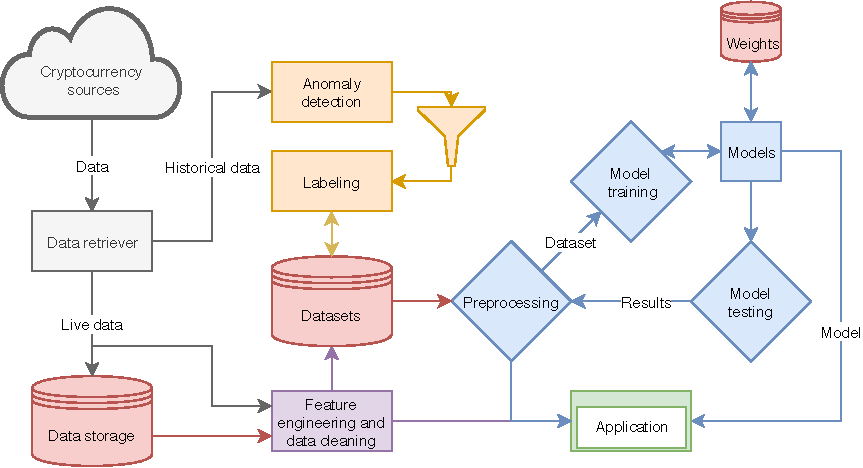
\includegraphics[width=\textwidth]{overview.pdf}
    \caption[\project's architecture]{\project's architecture. The first processing stage in the pipeline is the data retriever, and it pushes data to the feature engineering and data cleansing stage to prepare the data for \ac{ml}. Historical data that spans over the period where data is collected gets fetched and pushed through an anomaly detection algorithm that detects \acp{pd}. The labeled data gets first preprocessed, then either pushed to train a model or, if deployed, to straightly to a trained model that can make predictions.}
    \label{fig:overview}
\end{figure}

The first step in the pipeline pulls data over the internet from sources that has information regarding \acp{pd} in cryptocurrencies. The data is mostly incomplete by lacking trends or being unprocessed, making it potentially challenging to train a model and obtain good results. This process is tedious because sources tend to have different request rates, \acp{api}, and the data can have various formats like \ac{json} or \ac{xml}.

The next step branches the retrieved data in two, live and historical data. Since we are trying to detect \acp{pd} in real-time we need to store live data continuously. When we have captured a compelling amount of \acp{pd}, we use an anomaly detection algorithm~\cite{P&D_to_the_moon} to detect \acp{pd} in the gathered live data. This algorithm is not compliant with live data, so we need to pull aggregated historical data that span throughout the collected live data. As previously mentioned, anomaly detection algorithms tend to have a high number of false positive compared to true positive. Thus, we need to remove these false positives and keep the true positive manually.

The input data ultimately determine the performance of a \ac{ml} deep learning model~\cite{mike_voets}. Training a model with the raw gathered live data is ineffective. Hence, we need to define a new convenient dataset containing features created by processing the collected live data; this is a highly critical process and will later determine the classification performance of the deep learning model. The gathered live data also need to undergo a cleansing process as a portion of it presumably are not relevant \ac{pd} information.

With filtered anomalies containing \ac{pd}, we create a labeled dataset and train our model. Obtaining good classification results depends, as mentioned, on the features, but also how we decide to preprocess the dataset. Typical preprocessing strategies include dimensionality reduction and normalization. Having a labeled preprocessed dataset, we can finally begin to train the deep learning model. This a cyclical and a long process, as it requires many trial and error attempts to find the optimal weights for the model. In each cycle, we store the model's weights because it is not always the case that each iteration will improve the classification performance of the model.

For applications to utilize \project, they need to select a model and let live data flow through the same processing stages as the dataset that was used to train the model.

\section{Internal Components}

\subsection{Retrieving Data}
Every problem that is solved using \ac{ml} requires data. The more data, the better the results will be when training a model. As previously mentioned, cryptocurrency sources like exchanges produce time series data containing, e.g., price and volume of a coin. The data is continuously produced in a limited amount with proportion to time.

Since we want to detect \acp{pd} on exchanges in real-time, the nature of the data we want to make classifications on is live fine-grained data so that the model can detect them as early and accurately as possible. Aggregated historical data is too coarse-grained because exchanges generally only allow a discrete time interval selection of data where the smallest is typically one minute. The duration where they start to where they peak varies from a few seconds to a maximum of ten minutes~\cite{P&D_MIT_crypto, P&D_to_the_moon}, and the ability to make accurate predictions with one-minute data is questionable.

Training a model in real-time by pulling data is impractical because it will not be labeled. In addition, sources can only produce a limited amount of data at a time which will create a bottleneck of data supply to the model. To cope with these problems, we have to pull and store current live data continuously; this is a time-consuming process for we have to wait until we have captured enough \ac{pd} events before we can start training. If anything fails, we may have to start all over again as we are missing out on trends, which results in noisy data.

From the reinforcers field in \autoref{tab:pd_indicators}, we see that we have to fetch data from various sources. An exchange alone does not produce data regarding a coin's capitalization, nor a coin's price on a different exchange. Sources other than exchanges produce such metadata of coins, while exchanges only produce internal trading data.

\subsubsection{Master Slave Approach}
We shape our data retriever like a master/slave model. \autoref{fig:ms} is an example that illustrates our data retriever with a master and its three data-pulling slaves. Each slave in our data retriever is assigned a source that can e.g. be an exchange. The communication between slaves and the master is as follows. The master broadcasts a pull signal to the slaves, and they pull the data from their assigned source. Then the master gathers the data from them and parses it, and augments all the data into a single sample. Each sample the master generate gets stored. This procedure takes effect in a fixed interval. By letting the master signalize the slaves to retrieve data simultaneously, we collect clean time-series data where each sample's time gap is circa equal. 

\begin{figure}[hbt!]
    \centering
    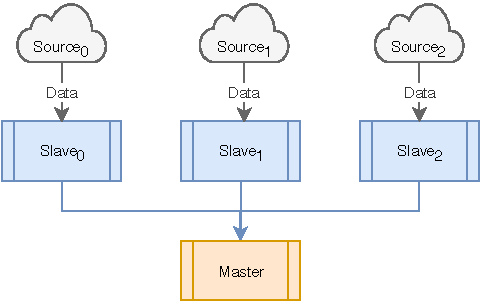
\includegraphics[width=0.8\textwidth]{ms.pdf}
    \caption[\project's data retriever]{\project's data retriever. The slaves are assigned a source. The master, in a fixed interval, broadcasts a pull signal to the slaves, and the slaves fetch data from their designated source. Soon as the slaves complete their task, the master gathers the result from them.}
    \label{fig:ms}
\end{figure}

\subsubsection{Collecting Trading Data From Multiple Markets}
Previous work in detection of \acp{pd}~\cite{P&D_to_the_moon} estimated that $1.6$ \acp{pd} is carried out daily per market, and this raises several problems. First, multiple exchanges have the same market, and we can not know which exchange they target unless we have prior knowledge from their \ac{pd} group. Second, gathering data from a single market is inadequate, the data retriever would with an estimate capture $48$ \ac{pd} occurrences, if it gathered every \ac{pd} event on a single market for a whole month. Training a model with $48$ \ac{pd} instances is inadequate. 

To alleviate these problems, we collect data for all markets from a single exchange to make sure we obtain as many \ac{pd} events as possible. We assume the \ac{pd} pattern remain the same across markets. Otherwise, we may run into trouble when training our model by having too few samples with various patterns. Also, by training the model using data from all the markets generalizes the model, which makes the model compliant to new markets who are excluded during training.

\subsubsection{Feature Description}
From the \ac{pd} indicators described in \autoref{tab:pd_indicators}, we define a set of features in \autoref{tab:features}. We believe that these features contain the necessary information for a model to detect \acp{pd}. Features like a coin's capitalization are available at \href{https://coinmarketcap.com/}{CoinMarketCap}, while trading data like order book and \ac{ohlcv} values are available at exchanges. A specific feature that is challenging to attain is aggregated \ac{ohlc} values from multiple exchanges, as this requires us to request multiple exchanges simultaneously and aggregate the data.

\begin{table}[ht]
    \centering
    \begin{tabular}{p{0.30\textwidth} p{0.70\textwidth}}
        \hline
        \textbf{Feature} & \textbf{Description}\\
        \hline
        \ac{ohlcv}                      & Latest \ac{ohlcv} values.\\
        \hline
        \ac{ohlcv} multiple exchanges   & Aggregated \ac{ohlcv} values from multiple exchanges.\\
        \hline
        Order book                      & Level $1$ (aggregated price and volume) order book with a depth of $5$.\\
        \hline
        Order book imbalance            & The imbalance between bids and asks orders and quantity.\\
        \hline
        Coin capitalization ratio       & Coin capitalization ratio.\\
        \hline
        Volume traded                   & Base and quote volume traded for the last $24$ hours.\\
        \hline
        number of trades                & Number of completed trades for the last $24$ hours.\\      
        \hline
        bid and ask price               & Best bid and ask price for the last $24$ hours.\\
        \hline
        bid and ask volume              & Best bid and ask quantity for the last $24$ hours.\\
        \hline
        Average price                   & Average price for the last $24$ hours.\\
        \hline
        symbol-pair exchange rate       & The rate of how many exchanges that lists the symbol-pair.\\ 
        \hline
        Time                            & Unix timestamp.\\
        \hline
    \end{tabular}
    \caption[Features description]{Feature description}
    \label{tab:features}
\end{table}


\subsection{Preparing Data}\label{sec:prep}
Data preparation is an important task. In practice, it has shown that data cleaning and preparation takes approximately $80\%$ of the total data engineering effort, as it requires solid domain knowledge of the subject. Data preparation comprises those techniques concerned with analyzing raw data to yield quality data. Some of the techniques are; data collecting, data integration, data transformation, data cleaning, data reduction, and data discretization~\cite{zhang2003data}.

Because of this, we fetch data from multiple markets to create a generalized model; we must prepare the data and make it equally scaled. Markets are distinct, and they have different trading price and volume, which makes predictions with these raw numerical values nonviable. If a \ac{pd} occurs on a coin with a low cost, and the price is increasing at $300\%$. Despite the high increase and profit, the coin is still almost worthless compared to other expensive coins, and the numerical price increase do not necessarily need to be that high. On the other hand, if the price of an expensive coin increase with only $1\%$, the numerical value can still be high despite the low percentage increase. Since the model is generalized, it is weighing each market equally. So using raw data like the price is infeasible, as a low price change in an expensive market reflects a massive change in a cheap market. Thus, we must transform all these raw market specific values to values that are general across markets.

\subsubsection{Data Cleansing}
Data cleaning, also called data \emph{cleansing} or \emph{scrubbing}, deals with detecting and removing errors, inconsistencies, and unproductive features from data in order to improve the quality of data~\cite{data_cleaning}. Fetched data from exchanges includes additional features not defined in \autoref{tab:features}. These features are removed as they add nothing of value. Instead, they increase the number of dimensions and makes the data more complex.

Markets with little or no activity may have intervals containing \emph{zero-data}. For example, if no investors have bought or sold assets in a specific interval, the exchanges tend to set the trading values to zero. These zero-values create significant spikes in the trend which we must address; otherwise, they disrupt the data. Besides, having zero-data does not make any sense, if the price is recorded to be zero, it means that the coin is free, which it is not.

We substitute every value that is zero by linearly interpolating each of them. Linear interpolation involves estimating a new value by connecting two adjacent known parameters with a straight line~\cite{interpolate}. These two known parameters are non-zero values that are adjacent on each side of the zero-value. Thus, we form \autoref{eq:interpolation} with the known parameters $(x_1, y_1)$ (previous non-zero value) and $(x_2, y_2)$ (next non-zero value), $y$ is the new value for some zero-value in point $x$.

\begin{align}\label{eq:interpolation}
    y = y_1 + (x - x_1) \frac{y_2 - y_1}{x_2-x_1}
\end{align}

\subsubsection{Feature Engineering}
Feature engineering is the process of using domain knowledge of the data to create features that make \ac{ml} algorithms work. Feature engineering is fundamental to the application of machine learning and is both challenging and expensive, but when done correctly, it can result in wonders~\cite{feature_engin}.

\subsubsection{Processing Order Book}
As previously mentioned in \autoref{sec:pump_groups}, \ac{pd} organizers invest in the market before the \ac{pd} without raising the price. We believe that the order book in said market oscillates before the pump, and especially during the pump. Therefore, we calculate an imbalance between sell and bid orders; this is a multidimensional problem considering an order book contains both a list of prices along with its volume, as we saw in \autoref{tab:order_book}. \autoref{eq:imbalance} reduces this multidimensional problem to a single value. $p$ and $v$ is respectively the lists of prices and volumes, and the annotations $a$ and $b$ denotes ask and bid orders. If \autoref{eq:imbalance} yields a value between $(0,1)$, it emphasize the bidders, if it yields a value between $(1, \infty]$ then askers, and if it yields $1$ the order book is balanced.

\begin{align}\label{eq:imbalance}
    imbalance = 
    \frac{
    \begin{bmatrix}
        p^a_1 \\
        \vdots \\
        p^a_n
    \end{bmatrix}
    \cdot
    \begin{bmatrix}
        v^a_1 \dots v^a_n
    \end{bmatrix}
    }{
    \begin{bmatrix}
        p^b_1 \\
        \vdots \\
        p^b_n
    \end{bmatrix}
    \cdot
    \begin{bmatrix}
        v^b_1 \dots v^b_n
    \end{bmatrix}
    }
    = \frac{\langle P_a, V_a \rangle}{\langle P_b, V_b \rangle}
\end{align}

\subsubsection{Processing Trading Data}
We process trading data such as price and volume by calculating the \ac{poc}. By doing this, we transform these values in each market to the same scale, and eliminate the need for the model to adjust to raw values. For example, if the coin ETH increase by \$$10$ from a starting value of \$$100$, and the coin ADA increase by \$$5$ from a starting value of \$$50$, then both coins increase by $10$\%.

\begin{align*}%\label{eq:pct}
    pct(x, v_\gamma) = \frac{x - v_\gamma}{x}
\end{align*}

We define the function $pct$ as in \autoref{eq:pct} to calculate the \ac{poc}. It calculates the percentage change in point $x$ concerning a previous value $v$ with a time lag $\gamma$. We consider $x$ and $v$ to be a single value like the price or volume, while $\gamma$ indicates moving backward in time from point $x$. We must be vigilant when using this technique, if the data contains values that are zero, we might perform a zero-division that can clutter with the data unpredictably. However, since we scrubbed the data first and removed zero-values, this should not be a concern.

\subsubsection{Processing Time}
According to \cite{P&D_anatomy}, the time is essential when classifying \acp{pd}. They are typically executed on the hour (6:00, 7:00, etc.) because organizers usually does not choose a random time. Data retrieved from sources are getting timestamped, and we can take advantage of these timestamps to check whether data was generated at the hour or not. The function $x_\delta$ transforms a Unix timestamp\footnote{Unix timestamp is a way to track time as a running total of seconds since the Unix Epoch, January 1st, 1970.} to a value in the interval $[0, 1)$. The closer $x_\delta$ is to the margins, the closer the time is to the hour, but since $0$ and $1$ symbolizes the same, we have to process it further before we can use it as a valuable feature.

\begin{figure}
    \centering
    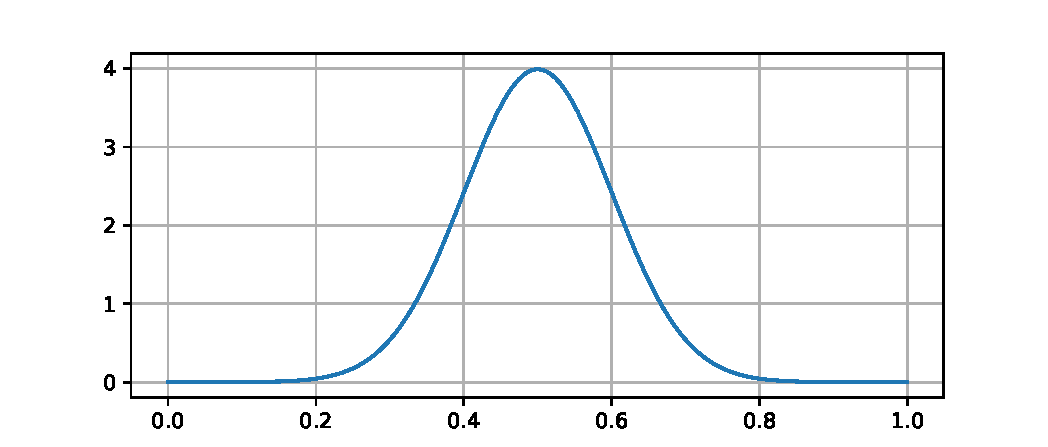
\includegraphics[width=\textwidth]{time.pdf}
    \caption[\project's time curve]{Gaussian distribution $t$ from \autoref{eq:gaus} with the parameters $\sigma=0.1$ and $\mu=0.5$. The curve describe how close a given time-parameter $x$ is on the hour (6:00, 7:00, etc.).}
    \label{fig:unixtime}
\end{figure}

\begin{equation}\label{eq:unix_time}
    x_\delta(x_{\textbf{unix}}) = \frac{x_\textbf{unix}\mod 3600}{3600}
\end{equation}
\myequations{UNIX timestamp scaling}

\begin{align}\label{eq:gaus}
    t(x_\delta, \mu, \sigma) &= \frac{1}{\sqrt{2\pi\sigma^2}} e^{-\frac{x_\delta-\mu}{2\sigma^2}}, \quad \text{where}
    \begin{cases}
    \mu = 0.5 \\
    \sigma = 0.1 
    \end{cases}
\end{align}
\myequations{Data preparation - Time}

We define a Gaussian distribution function $t$ (\autoref{eq:gaus}) with the parameters $\mu=0.5$ and $\sigma=0.1$ which creates the graph illustrated in \autoref{fig:unixtime}. The graph shows when given $t$ a $x_\delta$ close to $0$ or $1$ (6:00, 7:00, etc.), $t$ returns a value close to $0$, but when given $0.5$ (6:30, 7:30, etc.) it returns a value close to $4$. $t$ demonstrate that we can separate data by how close it was generated to the hour. Also, we can always tweak $\sigma$ to adjust the width of the curve Adjusting the curve allows us to be more strict, the wider the curve, the more strict.

\subsection{Collecting Pump-and-Dumps}
Manually collecting \ac{pd} events from chat applications to label our collected data. seems infeasible in the long run. Although Livshits and Xu~\cite{P&D_anatomy} hand-picked $220$ pump-events from July to November in 2018 from $358$ different Telegram groups to train a Random Forest model, they still missed a lot of other executed \ac{pd} schemes as there are numerous chatting applications and private organizers~\cite{blockonomi}. Also, searching for \ac{pd} events is a time-consuming process, and incorrect labeling occurs when we lack membership to all of \ac{pd} groups, which results in suboptimal prediction capacity~\cite{label_noise}. We also have to be aware of whether a \ac{pd} was successfully executed or not; labeling failed attempts as positive only contributes to label noise. Instead of manually collecting \acp{pd} from groups in chatting applications, we believe that it is possible to hand-pick \acp{pd} by \emph{reasoning abductively} with the help of an anomaly detection algorithm to pinpoint suspicious time intervals in historical data.

The anomaly detection algorithm identifies local \emph{contextual anomalies} based on fixed recent history called a \emph{sliding time window}. A sliding window is a period that stretches back in time (lag factor) from the present containing events at specified intervals. The event intervals can overlap with each other, or they can be disjunct. As events exceed the lag factor, they fall out of the sliding window, and they are no longer matching against the rules applied to the sliding window~\cite{redhat}. With a sliding window, we can compare values in a given period, contrary to using single values, which alone does not yield much information in sequence data.

The anomaly detection algorithm is proposed by Kleinberg and Kamps~\cite{P&D_to_the_moon}, which is inspired by previous research in \ac{dos} attacks~\cite{dos}. It is a threshold based technique to find a suspicious increase in price and volume of a coin. If the price and volume in a specific interval are higher than some threshold, then the interval is flagged as anomalous and warrants further investigation.

\subsubsection{Price Anomaly}
We compute the price anomaly threshold by the simple moving average listed in \autoref{eq:price_anomaly}. $\mu_\gamma^p$ of \ac{ohlcv} values denoted $x$ with a lag factor $\gamma$ multiplied with a given percentage increase $\epsilon_p$. We consider $x$ and $\gamma$ as \ac{ohlcv} objects, and $x-\gamma$ indicates moving backwards in the sliding time window by a factor of $\gamma$~\cite{P&D_to_the_moon}. If the highest registered price in $x$'s period is greater than the computed threshold, we flag the period as anomalous.

\begin{align}
    \mu_\gamma^p(x) &= \frac{\sum^x_{i=x-\gamma} x_{close}}{\gamma}\\
    price\_anomaly(x)&=
    \begin{cases}
        True  & \text{if $x_{high} >    \epsilon_p \cdot \mu_\gamma^p(x)$}\\
        False & \text{otherwise}
    \end{cases}
\end{align}

\subsubsection{Volume Anomaly}
Calculating the volume anomaly threshold is almost identical to calculating the price anomaly. We are only substituting $x_{closing}$ and $x_{high}$ with $x_{volume}$. The resulting formula is listed in \autoref{eq:volume_anomaly}.

\begin{align*}
    \mu_\gamma^v(x) &= \frac{\sum^x_{i=x-\gamma} x_{volume}}{\gamma}\\
    volume\_anomaly(x)&=
    \begin{cases}
        True  & \text{if $x_{volume} >    \epsilon_v \cdot \mu_\gamma^v(x)$}\\
        False & \text{otherwise}
    \end{cases}
\end{align*}
\myequations{Anomaly - Volume}

\subsubsection{Filtering Anomalies}
Anomaly detection algorithms have a high false alarm rate~\cite{grill2017reducing}, which makes them difficult to use. And since we want to use the anomalies we collected to train a model with, it is imperative to remove false \acp{pd}. Otherwise, training a model with false \acp{pd} will make the model perform poorer, and result in even higher occurrences of false positives. Therefore, we manually remove all the false-positive anomalies, but removing them requires prior knowledge of \acp{pd}, which we do not have.

The anomaly detection algorithm checks whether \acp{pd} occurs in a specific interval. We visualize one-minute klines that span over intervals that are flagged anomalous. By plotting these values we can compare them to real \acp{pd}, like the ones seen in \autoref{fig:pd-gxsbtc}. A market's capitalization, if the pairing coin is BTC, is also helpful when filtering \ac{pd}. E.g. if the anomaly detection algorithm flagged a suspicious interval in the ETH-BTC market, and it visually looks like a \ac{pd}, then it still would with a high likelihood not be a \ac{pd} as ETH is the coin with the second highest capitalization~\cite{coinmarketcap_eth}.  As this would break the pattern where the organizers target coin with low capitalization. Further helpful characteristics regarding \acp{pd} is described in \autoref{tab:pd_characteristics} and \autoref{tab:pd_indicators}.

\subsubsection{Labeling Pump-And-Dumps}
With the new generated features from collected data and filtered anomalies containing \acp{pd}, we can label the new features and define a dataset. But first, the filtered anomalies are still intervals where a \ac{pd} occurred, and not precisely when it occurred. So, we need to precisely define where every \ac{pd} started and ended, before labeling.

Because the purpose of \acp{pd} is to raise the price of an asset, the point where the price change is highest in an interval is where the \ac{pd} peaked. If we have the peak of a \ac{pd}, we can search from the peak and down the descending slopes on each side of it. Left side will be the pump and the tight side will be the dump. From each side, we search until the change in price is equal or smaller than $0$. Finally, when have defined the start and end of every \ac{pd}, we label all the new features positive where there are \acp{pd}, and negative otherwise.

\subsection{Deep Learning}
This section describes the model we use to detect \acp{pd}, and how we process data, trains the model, and which metrics we should use to evaluate the model. These steps are an iterative process, where each iteration tend to improve the model.

\subsubsection{Preprocessing}
Before training a model with the generated dataset, we transform the dataset by \emph{normalizing} the features as they have various scales. Then, a common technique is to \emph{normalize} the input data. Normalization creates new values from the dataset, but still maintain the general distribution and ratios in the source data while keeping values within a scale applied across all used features~\cite{normalize_data}. Also, normalization of data occasionally improves the performance of the model by accelerating convergence speed of its weights during training~\cite{sola1997importance, normalize_google}.

There are several ways to normalize data, and the normalization technique used may have an impact on the performance of the model. Since \acp{pd} are anomalies, some features like percentage change in price and volume will make them look like outliers in the data. A traditional method called \emph{min-max} normalization is repeatedly used in detection of outliers~\cite{campos2016evaluation, goldstein2016comparative}. This technique provides a linear transformation of the data~\cite{panda2014smoothing}, allowing us to keep the distance ratio, and it scales every value into the range $[0,1]$.

\begin{align}\label{eq:minmax}
    x_{ij}' = \frac{x_{ij} - \min(x_j)}{\max(x_j)-\min(x_j)} 
\end{align}

\autoref{eq:minmax} is the min-max normalization formula for a coefficient $x_{ij}$ in a dataset $x$. $x_j$ represents a column in a dataset with samples as row vectors.

\subsubsection{Model}
The model type we use to detect \ac{pd} is a \ac{lstm} network, illustrated in \autoref{fig:lstm}. This network contains \ac{lstm} cells in the hidden layer as we want the cells to have an internal state to remember the trend in data. We modeled the detection of \acp{pd} as a \emph{binary classification} problem, it is either positive (\ac{pd}) or negative (not \ac{pd}). Thus, in the output layer we only require a single perceptron to make the final classification.

\begin{figure}[ht]
    \centering
    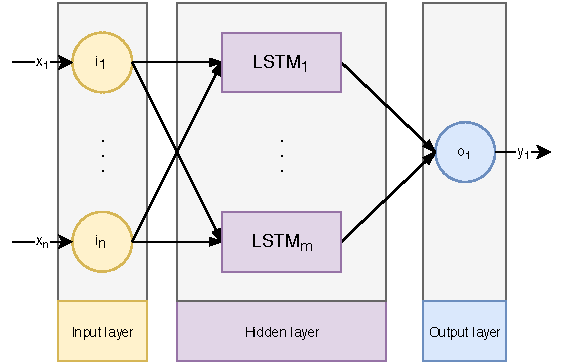
\includegraphics{lstm.pdf}
    \caption[\project's deep learning model]{structure of our model. The passive cells in the input layer propagate their input data $x$ to the first hidden layer that compose of \ac{lstm} cells. Then the cell's output in the hidden layers is the cell's input in the output layer. The last cell yields a prediction $y$.}
    \label{fig:lstm}
\end{figure}

\subsubsection{Training}
Before we start to train our model, we have to split the dataset into two sets, a training set, and a test set. The training set will we use to train the model, and the test will we use to evaluate the model. There is also a validation set that is used to fine-tune the hyperparameters during the training, but since there are so few \ac{pd} samples, we choose to avoid using a validation set and use those \ac{pd} samples we have to train our model and evaluate it.

As previously mentioned, \acp{pd} are anomalies, and that results in a significant class imbalance between positive and negative samples, which, when trained will make the model to overfit to the negative class and more or less ignore the positive class, it entirely depends on the distribution of them. Also, the academia is split concerning the definition, implication and possible solutions to this problem~\cite{tw_imbalance_2} making it currently ambiguous how to properly deal with it.

\begin{figure}[ht]
    \centering
    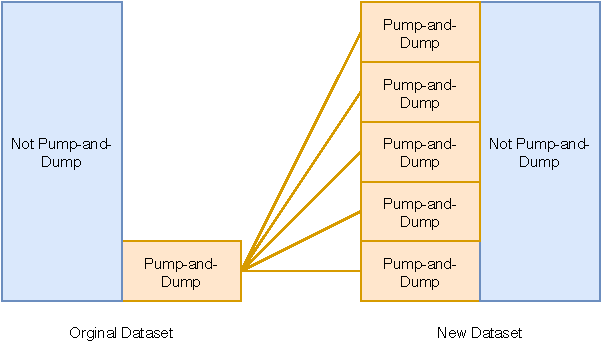
\includegraphics{oversampling.pdf}
    \caption[Oversampling dataset]{Oversampling (source\cite{tw_imbalance}). Involves duplicating a minority class (\ac{pd}) until the size is equal to the majority class (not \ac{pd}).}
    \label{fig:oversampling}
\end{figure}

We believe that we can solve our imbalance problem by using a technique called \emph{oversampling}, which \autoref{fig:oversampling} illustrates. Oversampling gathers all the samples from the minority class and duplicates them until the amount is approximately equal to the majority class. There is also a technique called \emph{undersampling}, that select random samples into a subset from the majority class until the size is equal to the number of samples in the minority class, but by using the oversampling technique, we can train our model with the whole dataset. With a balanced dataset, we can finally train our model.

Depending on the size of the dataset and number of epochs, training a model takes a really long time. Thus, after each training, we store the model and all its weights and other internal parameters.

\if0
\subsubsection{Evaluation}
After the training phase, we evaluate the model by classifying all the samples in the test dataset. The metrics, \emph{precision}, \emph{tp-rate}, and \emph{fp-rate} are probably the most important metrics to optimize when it comes to detection of anomalies. Sometimes, finding the best parameters is done by multiple trials and errors attempts. Adjusting the parameters like the number of, hidden layers, cells, and epochs might improve said metrics. Also, shuffling samples may improve the model as we train with a few numbers of original \acp{pd} samples.
\fi

%\newpage
\section{Phases}
Till now, in this chapter, we have described each component in \project. As we mentioned in \autoref{ch:background}, when we have trained a model, we can feed the model with real-time data and it will classify whether the given data is a \ac{pd} or not. This allows us to dismiss numerous components which are not needed anymore. They only need to be present during the training phase. So we can divide \project into two phases, a training phase, and a deployment phase. In the training phase, \project depends on all the components except the application box in \autoref{fig:overview}. In the deployment phase, there are only a few components needed.

\subsection{Deployment}
\autoref{fig:pipe} illustrates the components that are needed in this phase. The first component, the data retriever, function precisely like described above, it fetches data and pushes it further down the pipeline. The next two stages need to retain their internal parameters from the training phase. Otherwise, the model will classify input data that is processed differently from what it was trained with. 

\begin{figure}[ht]
    \centering
    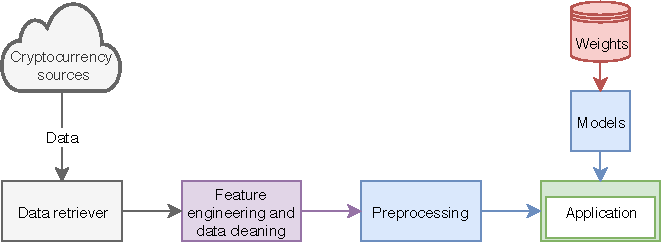
\includegraphics{pipe.pdf}
    \caption[\project's deployment pipeline]{deployment pipeline. The data retriever fetch data and pushes it further to create new features. The new features get normalized and given to the application. With data and a model, the application can make a prediction.}
    \label{fig:pipe}
\end{figure}

In order for applications to use \project, they need to select a model that was generated during the training phase. With both a trained model and real-time data, they can potentially predict whether the given input data is a \ac{pd} or not.